% Soubory musí být v kódování, které je nastaveno v příkazu \usepackage[...]{inputenc}

\documentclass[%
%  draft,    				  % Testovací překlad
  12pt,       				% Velikost základního písma je 12 bodů
  %a4paper,    				% Formát papíru je A4
	t,                  % obsah slajdů nebude centrovaný, nýbrž budou začínat od hora
%  oneside,      			% Jednostranný tisk (výchozí)
%% Z následujicich voleb lze použít maximálně jednu:
%	dvipdfm  						% výstup bude zpracován programem 'dvipdfm' do PDF
%	dvips	  						% výstup bude zpracován programem 'dvips' do PS
%	pdftex							% překlad bude proveden programem 'pdftex' do PDF (výchozí)
	unicode,						% Záložky a informace budou v kódování unicode
%% Z následujících voleb lze použít jen jednu:
%english,            % originální jazyk je angličtina
czech ,             % originální jazyk je čeština (výchozí)
%slovak,             % originální jazyk je slovenčina
aspectratio=169
]{beamer}				    	% Dokument třídy 'zpráva'

\usepackage[utf8]		%	Kódování zdrojových souborů je v UTF-8
	{inputenc}					% Balíček pro nastavení kódování zdrojových souborů

\usepackage{graphicx} % Balíček 'graphicx' pro vkládání obrázků
											% Nutné pro vložení log školy a fakulty

\usepackage[
	nohyperlinks				% Nebudou tvořeny hypertextové odkazy do seznamu zkratek
]{acronym}						% Balíček 'acronym' pro sazby zkratek a symbolů
											% Nutné pro použití prostředí 'seznamzkratek' balíčku 'thesis'

%% Balíček hyperref vkládá beamer automaticky
%\usepackage[
%	breaklinks=true,		% Hypertextové odkazy mohou obsahovat zalomení řádku
%	hypertexnames=false % Názvy hypertextových odkazů budou tvořeny
%											% nezávisle na názvech TeXu
%]{hyperref}						% Balíček 'hyperref' pro sazbu hypertextových odkazů
%											% Nutné pro použití příkazu 'nastavenipdf' balíčku 'thesis'

\usepackage{pdfpages} % Balíček umožňující vkládat stránky z PDF souborů
                      % Nutné při vkládání titulních listů a zadání přímo
                      % ve formátu PDF z informačního systému

\usepackage{enumitem} % Balíček pro nastavení mezerování v odrážkách
  \setlist{topsep=0pt,partopsep=0pt,noitemsep}

\usepackage{cmap} 		% Balíček cmap zajišťuje, že PDF vytvořené `pdflatexem' je
											% plně "prohledávatelné" a "kopírovatelné"

\usepackage{upgreek}	% Balíček pro sazbu stojatých řeckých písmem
											% např. stojaté pí: \uppi
											% např. stojaté mí: \upmu (použitelné třeba v mikrometrech)
											% pozor, grafická nekompatibilita s fonty typu Computer Modern!

\usepackage{dirtree}		% sazba adresářové struktury

\usepackage[formats]{listings}	% Balíček pro sazbu zdrojových textů
\lstset{
    language=[LaTeX]{TeX},	% definice použitého jazyka
    basicstyle=\ttfamily,	% definice základního stylu písma
    tabsize=2,			% definice velikosti tabulátoru
    inputencoding=utf8,
    %inputencoding=cp1250,      % pro soubory uložené ve standardním kódování Windows CP1250
    extendedchars=true,
    literate=%  definice symbolů s diakritikou
    {á}{{\'a}}1
    {č}{{\v{c}}}1
    {ď}{{\v{d}}}1
    {é}{{\'e}}1
    {ě}{{\v{e}}}1
    {í}{{\'i}}1
    {ň}{{\v{n}}}1
    {ó}{{\'o}}1
    {ř}{{\v{r}}}1
    {š}{{\v{s}}}1
    {ť}{{\v{t}}}1
    {ú}{{\'u}}1
    {ů}{{\r{u}}}1
    {ý}{{\'y}}1
    {ž}{{\v{z}}}1
    {Á}{{\'A}}1
    {Č}{{\v{C}}}1
    {Ď}{{\v{D}}}1
    {É}{{\'E}}1
    {Ě}{{\v{E}}}1
    {Í}{{\'I}}1
    {Ň}{{\v{N}}}1
    {Ó}{{\'O}}1
    {Ř}{{\v{R}}}1
    {Š}{{\v{S}}}1
    {Ť}{{\v{T}}}1
    {Ú}{{\'U}}1
    {Ů}{{\r{U}}}1
    {Ý}{{\'Y}}1
    {Ž}{{\v{Z}}}1
}

%% Nastavení českého jazyka při sazbě v češtině.
% Pro sazbu češtiny je možné použít mezinárodní balíček 'babel', jenž
% použití doporučujeme pro nové instalace (MikTeX2.8,TeXLive2009), nebo
% národní balíček 'czech', který doporučujeme ve starších instalacích.
% Balíček 'babel' bude správně fungovat pouze ve spojení s programy
% 'latex', 'pdflatex', zatímco balíček 'czech' bude fungovat ve spojení
% s programy 'cslatex', 'pdfcslatex'.
% Varianta A:
\usepackage
  {babel}             % Balíček pro sazbu různojazyčných dokumentů; kompilovat (pdf)latexem!
										% převezme si z parametrů třídy správný jazyk
\usepackage{lmodern}	% vektorové fonty Latin Modern, nástupce půvoních Knuthových Computern Modern fontů
\usepackage{textcomp} % Dodatečné symboly
\usepackage[T1]{fontenc}  % Kódování fontu - mj. kvůli správným vzorům pro dělení slov
% Varianta B:
%\usepackage{czech}   % Alternativní balíček pro sazbu v českém jazyce, kompilovat (pdf)cslatexem!


\usepackage{graphicx}
\usepackage{caption}
\usepackage{subcaption}
\usepackage{amsmath}
\usepackage{mathtools}
\usepackage{alize} %moje styly
\usepackage{wrapfig}

\usepackage[%
%% Z následujících voleb lze použít pouze jednu
% left,               % Rovnice a popisky plovoucich objektů budou %zarovnány vlevo
  center,             % Rovnice a popisky plovoucich objektů budou zarovnány na střed (vychozi)
%% Z následujících voleb lze použít pouze jednu
%semestral						%	sazba zprávy semestrálního projektu
%bachelor						%	sazba bakalářské práce
diploma						 % sazba diplomové práce
%treatise            % sazba pojednání o dizertační práci
%phd                 % sazba dizertační práce
]{thesis}             % Balíček pro sazbu studentských prací
                      % Musí být vložen až jako poslední, aby
                      % ostatní balíčky nepřepisovaly jeho příkazy


%%%%%%%%%%%%%%%%%%%%%%%%%%%%%%%%%%%%%%%%%%%%%%%%%%%%%%%%%%%%%%%%%
%%%%%%      Definice informací o dokumentu             %%%%%%%%%%
%%%%%%%%%%%%%%%%%%%%%%%%%%%%%%%%%%%%%%%%%%%%%%%%%%%%%%%%%%%%%%%%%

%% Název práce:
%  První parametr je název v originálním jazyce,
%  druhý je překlad v angličtině nebo češtině (pokud je originální jazyk angličtina)
\nazev{Paralelizace Goertzelova algoritmu}{Parallelization of Goertzel algorithm}

%% Jméno a příjmení autora ve tvaru
%  [tituly před jménem]{Křestní}{Příjmení}[tituly za jménem]
\autor[Bc.]{Zdeněk}{Skulínek}

%% Jméno a příjmení vedoucího včetně titulů
%  [tituly před jménem]{Křestní}{Příjmení}[tituly za jménem]
% Pokud vedoucí nemá titul za jménem, smažte celý řetězec '[...]'
\vedouci[Ing.]{Petr}{Sysel}[Ph.D.]

%% Jméno a příjmení oponenta včetně titulů
%  [tituly před jménem]{Křestní}{Příjmení}[tituly za jménem]
% Pokud nemá titul za jménem, smažte celý řetězec '[...]'
% Uplatní se pouze v prezentaci k obhajobě
\oponent[prof.\ Ing.]{Zdeněk}{Smékal}[CSc.]

%% Označení oboru studia
% První parametr je obor v originálním jazyce,
% druhý parametr je překlad v angličtině nebo češtině
\oborstudia{Teleinformatika}{Teleinformatics}

%% Označení ústavu
% První parametr je název ústavu v originálním jazyce,
% druhý parametr je překlad v angličtině nebo češtině
\ustav{Ústav telekomunikací}{Department of Telecommunications} 

%% Rok obhajoby
\rok{Rok}
\datum{7.\,6.\,2017} % Uplatní se pouze v prezentaci k obhajobě

%% Místo obhajoby
% Na titulních stránkách bude automaticky vysázeno VELKÝMI písmeny
\misto{Brno}

%% Abstrakt
\abstrakt{
Technické problémy znemožňují neustále zvyšovat hodinové frekvence procesorů.
Jejich výkon tak v současné době roste díky zvyšování počtu jader.
To s sebou přináší nutnost nových přístupů pro programování takovýchto paralelních systémů.
Tato práce ukazuje, jak využít paralelismus k číslicovému zpracování signálu. Jako příklad zde bude uvedena implementace Geortzelova algoritmu s využitím výpočetního výkonu grafického čipu.
}{
Technical problems make impossible steadily increase processor's clock frequency.
Their power are currently growing due to increasing number of cores.
It brings need for new approaches in programming such parallel systems.
This thesis shows how to use paralelism in digital signal processing.
As an example, it will be presented here
implementation of the Geortzel's algorithm using the processing power of the graphics chip.
}

%% Klíčová slova
\klicovaslova{Goertzelův algoritmus, zpracování signálu, openCL, paralelní výpočet, GPU}%
	{Goertzel's algorithm, signal processing, openCL, parallel computing, GPU}

%% Poděkování
\podekovanitext{Rád bych poděkoval vedoucímu diplomové práce panu Ing.~Petru Syslovi, Ph.D.\ za odborné vedení, konzultace, trpělivost a podnětné návrhy k~práci.}  % do tohoto souboru doplňte údaje o sobě, o názvu práce...

%%%%%%%%%%%%%%%%%%%%%%%%%%%%%%%%%%%%%%%%%%%%%%%%%%%%%%%%%%%%%%%%%%%%%%%%

%%%%%%%%%%%%%%%%%%%%%%%%%%%%%%%%%%%%%%%%%%%%%%%%%%%%%%%%%%%%%%%%%%%%%%%%
%%%%%%     Nastavení polí ve Vlastnostech dokumentu PDF      %%%%%%%%%%%
%%%%%%%%%%%%%%%%%%%%%%%%%%%%%%%%%%%%%%%%%%%%%%%%%%%%%%%%%%%%%%%%%%%%%%%%
%% Při vloženém balíčku 'hyperref' lze použít příkaz '\nastavenipdf'
\nastavenipdf
%  Nastavení polí je možné provést také ručně příkazem:
%\hypersetup{
%  pdftitle={Název studentské práce},    	% Pole 'Document Title'
%  pdfauthor={Autor studenstké práce},   	% Pole 'Author'
%  pdfsubject={Typ práce}, 						  	% Pole 'Subject'
%  pdfkeywords={Klíčová slova}           	% Pole 'Keywords'
%}
%%%%%%%%%%%%%%%%%%%%%%%%%%%%%%%%%%%%%%%%%%%%%%%%%%%%%%%%%%%%%%%%%%%%%%%

% mod pro prezentaci, pouzije se tema (rozvrzeni) Darmstadt (nahradit podle libosti za jine)
\mode<presentation>{\usetheme{Darmstadt}}
% lze volat i \mode<presentation>{ \usetheme{Darmstadt} \usecolortheme{dove}}

\begin{document}

% snimek s titulni strankou vysazen bez hornich, dolnich a postranich list (volba plain),
% neni tak vysazen ani nadpis snimku
\vytvortitulku

% snimek s cili (zadanim) prace
\frame{  %2.snimek
   % nadpis snimku
   \frametitle{Cíle práce}
   % zde vlozit vlastni text k cilum (zadani) prace

		\begin{itemize}
			\item Seznámit se s možnostmi paralelního zpracování na počítačích typu PC a grafických procesorech.
			\item
			\item Prostudovat
principy a techniky paralelizace používané např. v prostředí Matlab nebo v rámci některé z knihoven pro paralelní
zpracování. 
			\item
			\item Seznámit s Goertzelovým algoritmem a navrhnout, jakým způsobem by bylo
možné jej urychlit pomocí paralelního zpracování.
			\item
			\item Porovnat výpočetní náročnost sekvenčního
a paralelního zpracování.
		\end{itemize}

}


% Zde vkladat dalsi snimky prezentace

% dalsi snimky prezentace
\frame{  % x-ty.snimek
     % nadpis snimku
    \frametitle{Knihovna openCL }
    

    


   
    
    \begin{itemize}

    \item Spravuje Kronos group
    \item
    \item Využití pro vícejádrová CPU, GPU, DSP a speciální zař.
    \item
    \item Obsahuje jazyk podobný C99, API, knihovny a runtime
    \item
    \item SIMD \& SPMD
    \item
    \item Model platformy
    \item
    \item Univerzálnost knihovny \& spolupráce s openGL
    \end{itemize}

}


% dalsi snimky prezentace
\frame{  % x-ty.snimek
     % nadpis snimku
    \frametitle{SIMD}
    

    
    
        \begin{figure}
		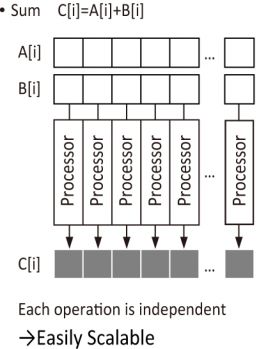
\includegraphics[scale=0.8]{obr/addvect}
		\end{figure}

}

\frame{  % x-ty.snimek
     % nadpis snimku
    \frametitle{Goertzelův algoritmus}
    
	\begin{itemize}
	\item Chceme $k$. složku spektra amplitud
	\item
	\item Číslicový filtr typu IIR
	\end{itemize}
	

	\begin{figure}
	   \centering
	    \begin{subfigure}[b]{0.5\textwidth}
	    \begin{footnotesize}
	    \begin{equation}
			\begin{aligned}
			\nonumber
				v_1[n+1] &= v_2[n], &&\\
				v_2[n+1] &= x[n]+2\cos{k\frac{2\pi}{N}}v_2[n]-v_1[n], &&\\
				y[n] &= v_2[n+1] -(\cos{k\frac{2\pi}{N}} -\jmag  		\sin{k\frac{2\pi}{N}}) v_2[n], &&\\
			\end{aligned}
		\end{equation}
		\end{footnotesize}
	  	\caption{\scriptsize Sada rovnic pro výpočet Goertzelovým algoritmem.\newline}
	  	%\label{obr:goertzelova2kanonicka}
	    \end{subfigure}
	    ~ %add desired spacing between images, e. g. ~, \quad, \qquad, \hfill etc. 
	      %(or a blank line to force the subfigure onto a new line)
	    \begin{subfigure}[b]{0.4\textwidth}
	    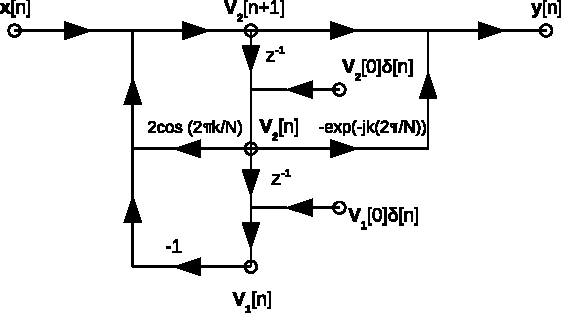
\includegraphics[scale=0.4]{obr/goertzel}
	  %\end{center}
	  	\caption{\scriptsize Graf signálových toků Goertzelova algoritmu ve 2. kanonické struktuře.}
	  	%\label{obr:goertzelova2kanonicka}
	    \end{subfigure}
	\end{figure}

}

\frame{  % x-ty.snimek
     % nadpis snimku
    \frametitle{Paralelní Goertzelův algoritmus}
    
    \begin{itemize}
    \item Variace stavové proměnné
    \item
    \item Počítání s $k$ hodnotami $x[n]$ současně\\
    \end{itemize}
      
    \begin{footnotesize}  
    \begin{equation}
    \nonumber
	\begin{multlined}
	v[n+k] = 
	\begin{pmatrix}
	v_1 [n+k] \\
	v_2 [n+k]
	\end{pmatrix}
	= A^k v[n] + \\
	\begin{pmatrix}
	A^{k-1}
	\begin{pmatrix}
	0 \\
	1
	\end{pmatrix}
	& A^{k-2}
	\begin{pmatrix}
	0 \\
	1
	\end{pmatrix}
	& A^{k-3}
	\begin{pmatrix}
	0 \\
	1
	\end{pmatrix}
	\dots
	\begin{pmatrix}
	0 \\
	1
	\end{pmatrix}
	\end{pmatrix}
	\begin{pmatrix}
	x[n] \\
	x[n+1]\\
	x[n+2]\\
	\vdots \\
	x[n+k]
	\end{pmatrix}
	=\\
	A^kv[n]+Dx[n,n+k]^T
	\end{multlined}
	\end{equation}
	\end{footnotesize}
	
	\tiny{kde $C_k = 2\cos{k\frac{2\pi}{N}}$} , 
	$A_k = \begin{pmatrix}
	0 & 1\\
	-1 & C_k\\
	\end{pmatrix}^k$

}


\frame{  % x-ty.snimek
     % nadpis snimku
    \frametitle{Program Sound Analyzer}
  
  	\begin{figure}
	   \centering
	   \nonumber	   
	   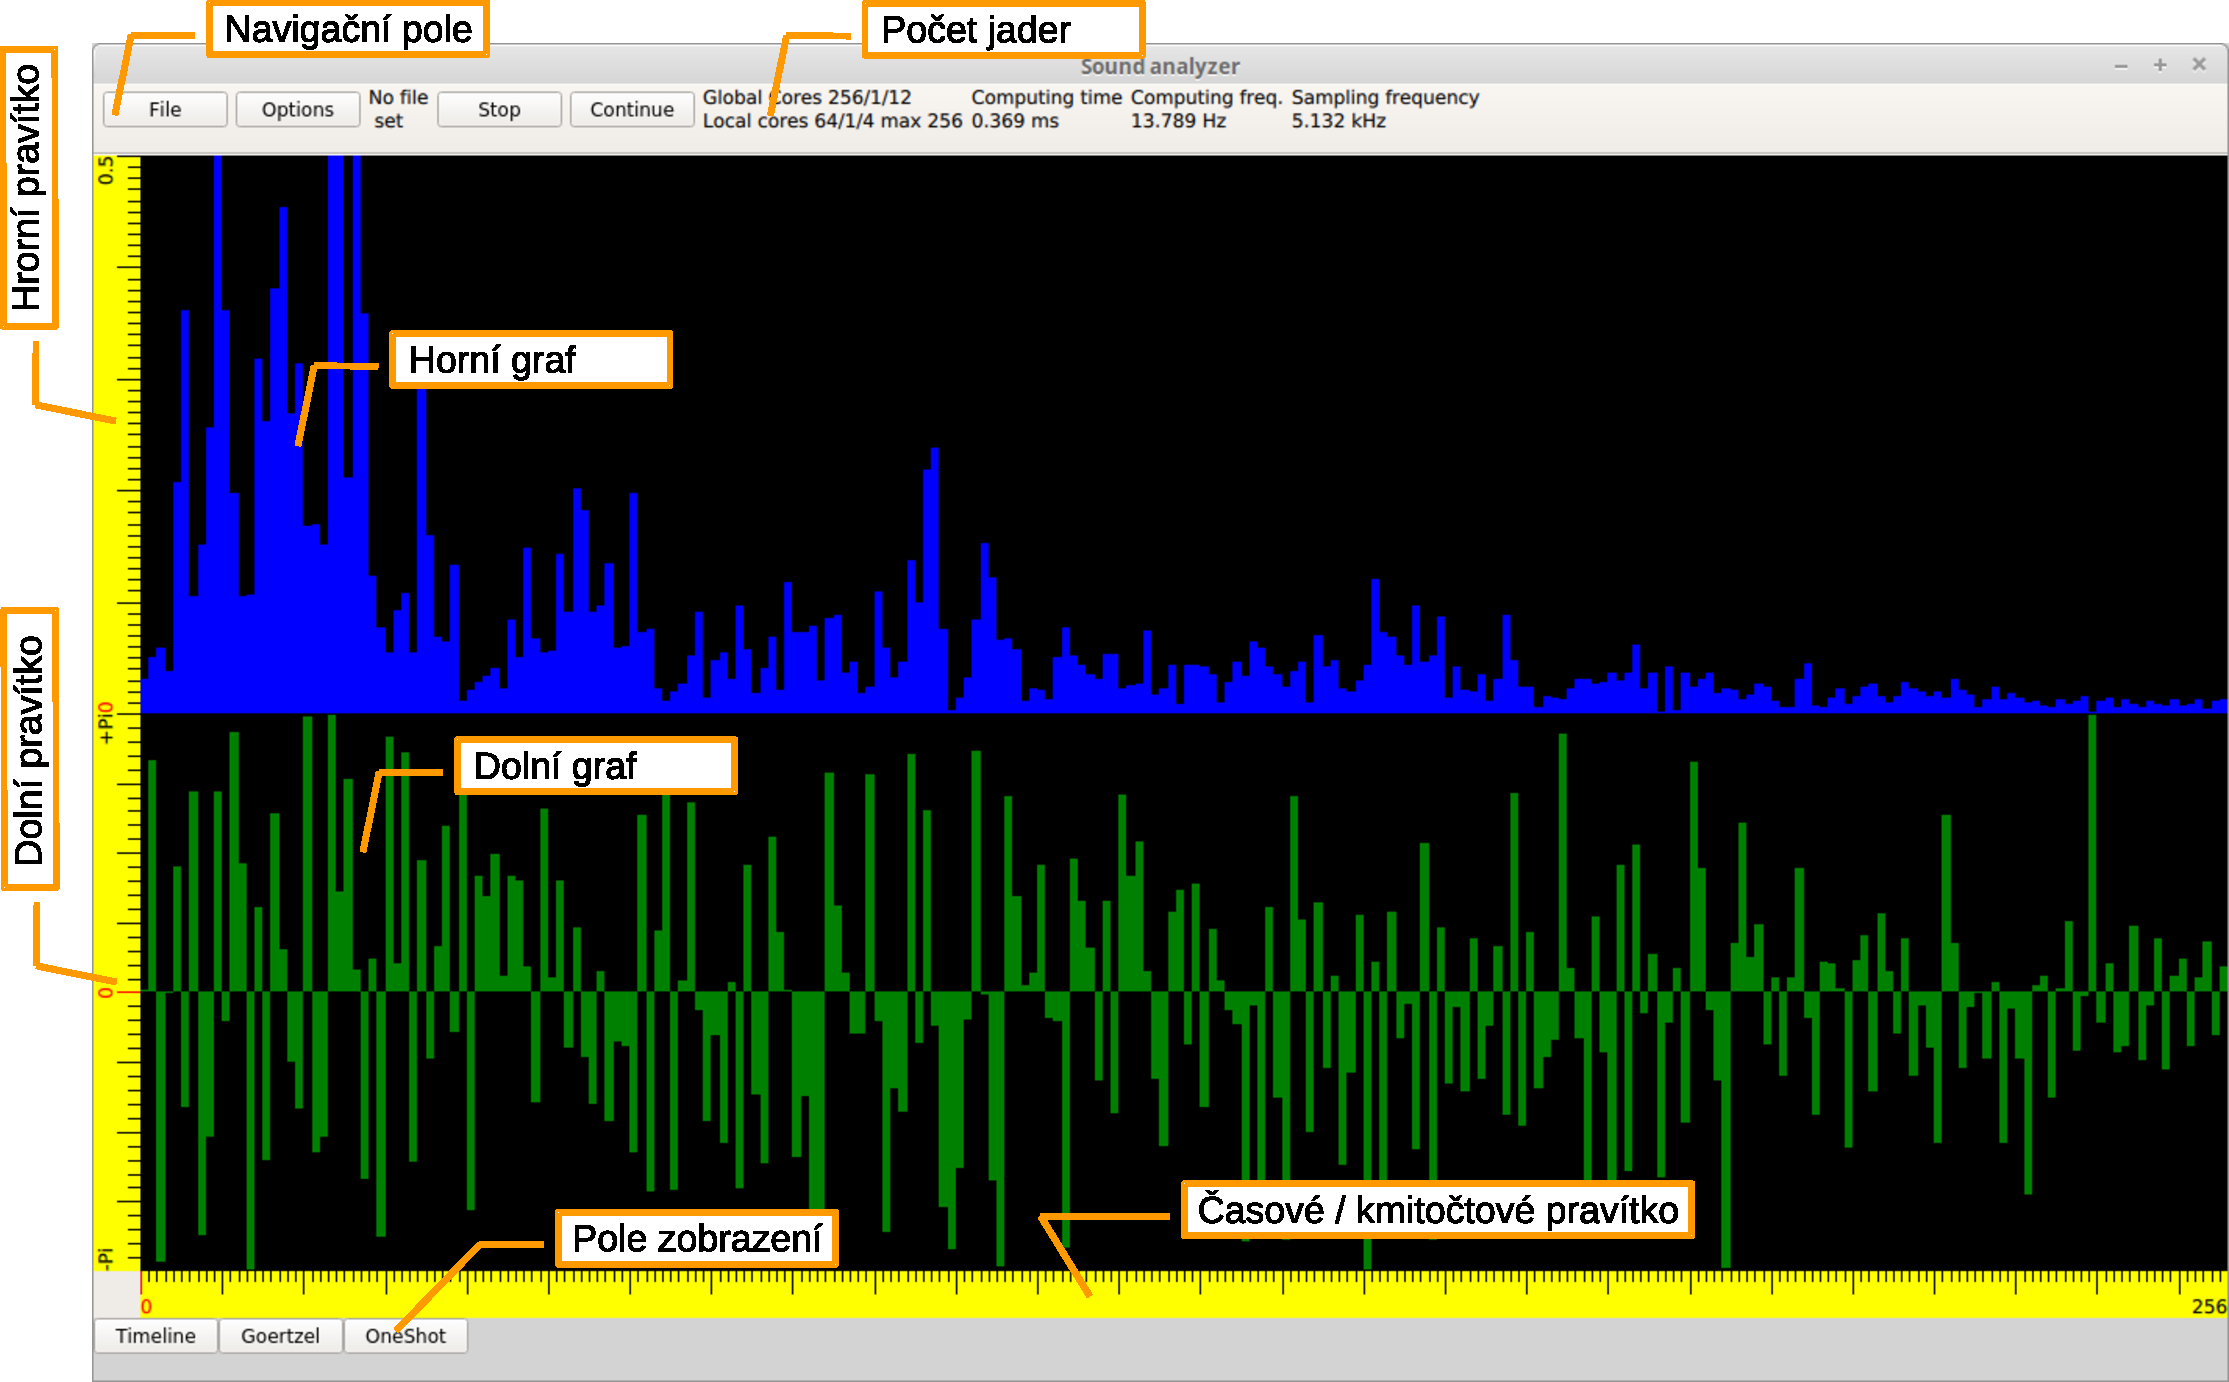
\includegraphics[scale=.25]{obr/manual2}
	   \caption{\scriptsize Program Sound Analyzer}
	\end{figure}

}


\frame{  % x-ty.snimek
     % nadpis snimku
    \frametitle{Struktura Programu Sound Analyzer}
  
  	\begin{figure}
	   \centering
	   \nonumber	   
	   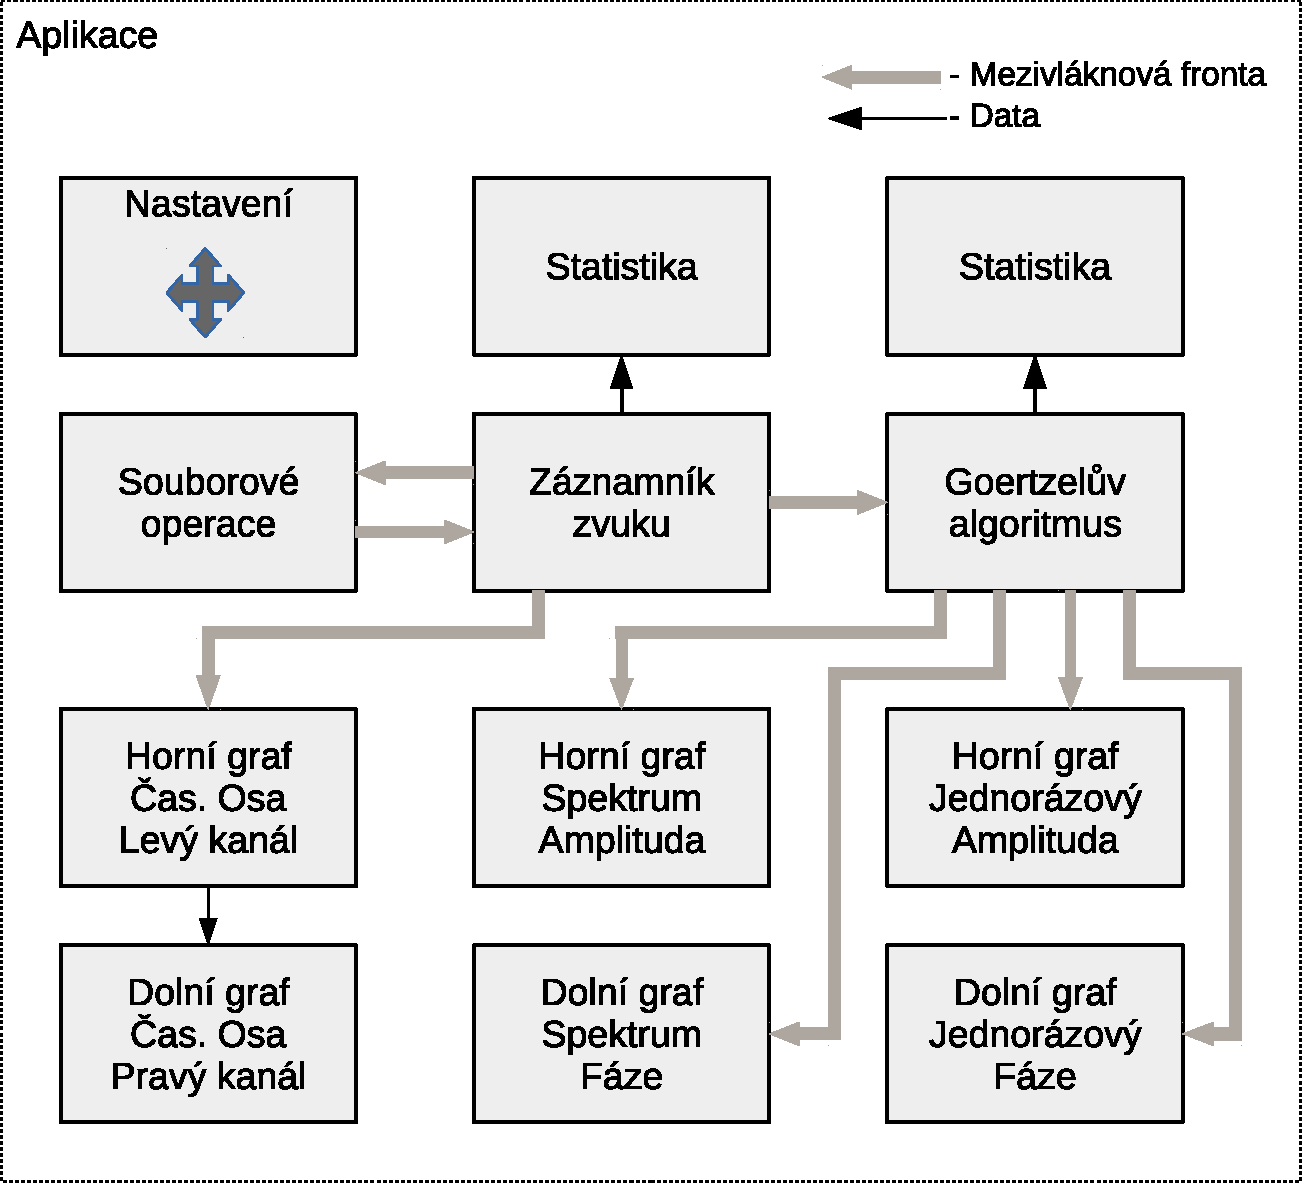
\includegraphics[scale=.3]{obr/SoundAnalyzeBlock3}
	   \caption{\scriptsize Struktura programu Sound Analyzer}
	\end{figure}

}

\frame{  % x-ty.snimek
     % nadpis snimku
    \frametitle{Doba provádění paralelního Goertzelova algoritmu}
    \begin{footnotesize}
    
\begin{table}
\centering

\begin{tabular}{|c|c|c|c|c|c|c|c|c|}
\hline
Kmit. & Segm. & Over- & Globální & Lokální & CPU & CPU & GPU & GPU\\
počet & délka & lap & NDRange & NDRange & doba & využití & doba & využití\\
$\left[ - \right]$ & $\left[ - \right]$ & $\left[ - \right]$ &$\left[ -/-/- \right]$ & $\left[ -/-/- \right]$ & $\left[ \mu s\right]$ & $\left[ \% \right]$ & $\left[ \mu s \right]$ & $\left[ \% \right]$\\
\hline
0&0&0&0/0/0&0/0/0&-&4,83&-&-\\
1&4&0&1/1/1&1/1/1&105&6,54&160&7,13\\
1&512&15872&1/1/64&1/1/64&230&5,3&410&5,0\\
16384&4&0&16384/1/1&1024/1/1&300&24,4&-&-\\
16384&512&15872&16384/1/64&16/1/64&61090&82,64&-&-\\
64&512&15872&64/1/64&16/1/64&690&5,25&-&-\\
64&512&15872&64/1/64&4/1/64&-&-&430&5,20\\
\hline
\end{tabular}
\caption{Naměřené hodnoty pro pro testovací počítač}
\end{table}

\end{footnotesize}
}

\frame{  % x-ty.snimek
     % nadpis snimku
    \frametitle{Měření využití jader na GPU}
    \begin{footnotesize}
\begin{table}
\centering

\begin{tabular}{|c|c|c|c|c|c|c|c|c|c|}
\hline
Lokální & \multicolumn{9}{c|}{Globální počet jader}\\
počet & 1 & 2&4&8&16&32&64&128&256\\
jader & &&&&&&&& \\
\hline
1&-&-&-&-&-&-&-&-&154\\
2&-&-&-&-&-&-&-&154&154\\
4&-&-&-&-&-&-&154&154&154\\
8&-&-&-&-&-&154&154&154&155\\
16&-&-&-&-&154&154&154&155&155\\
32&-&-&-&154&154&154&155&155&156\\
64&-&-&154&154&154&155&155&156&157\\
128&-&154&154&154&155&155&156&157&157\\
256&154&154&154&155&155&156&157&157&158\\
\hline
\end{tabular}
\caption{Naměřené hodnoty pro měření využití jader v \textup{$\mu s$}}
\end{table}

\end{footnotesize}
}

\frame{  % x-ty.snimek
     % nadpis snimku
    \frametitle{Výpočetní náročnost paralelního Goertzelova algoritmu}
    
    \begin{itemize}
    \item Funguje to, ALE
    \item
    \item Velká režie OpenCL
    \item
    \item Vhodné pro delší segmenty (1024 a více vzorků)
    \item
    \item Více úloh v těsném sledu -- nechávat data v paměti GPU 
    \item
    \item Aplikace by měla mít více vláken
    \item
    \item Neumíme rozdělit přímo fyzická jádra
    \end{itemize}
    

}

% predposledni snimek se zaverenym hodnocenim prace
\frame{ % predposledni snimek
 % nadpis snimku
 \frametitle{Závěr}
 % zde vlozit text zaveru prezentace
	
	\begin{itemize}
	\item Úprava vzorců pro paralelní sytém
	\item
	\item Realizace Goertzelova algoritmu a praktické aplikace
	\item
	\item Porovnání efektivity na skutečném zařízení
	\end{itemize}
}


% posledni snimek prezentace s podekovanim za pozornost
\frame{  % posledni snimek
   % nadpis snimku
   \frametitle{Závěr}
\vfill
\begin{center}
{\Huge Děkuji za pozornost!}
\end{center}
\vfill
}

\begin{frame}
	\frametitle{Otázky oponenta}
	% odpovedi na otázky oponenta
	\emph{Jaký je rozdíl mezi kmitočtovou charakteristikou LTI diskrétního systému a spektrem diskrétního signálu?}\\[2ex]
	
\begin{equation}
\nonumber
S_p(\jmag \omega) = \sum_{n=-\infty}^{\infty} s[n]\eul^{-\jmag \omega n} 	\Leftrightarrow H(\jmag \omega) = \sum_{m=-\infty}^{\infty} h[m]\eul^{-\jmag \omega m}
\end{equation}	\\
\begin{equation}
\nonumber
Y(e^{j\omega}) = H(e^{j\omega}) X(e^{j\omega})
\end{equation}	\\
$S_p(\jmag \omega)$ je spektrum signálu\\
$H(\jmag \omega)$ je spektrum impulsní charakteristiky
\end{frame}

\begin{frame}
	\frametitle{Otázky oponenta}
	% odpovedi na otázky oponenta
	\emph{Jak hodnotíte z hlediska času výpočtu a zátěže procesoru srovnání výpočtu několika složek spektra diskrétního signálu současně pomocí paralelizovaného Goertzelova algoritmu s výpočtem spektra pomocí FFT algoritmu?}\\[2ex]
	\begin{equation}
\nonumber
O(FFT) = O(N log_2 N ) 	\Leftrightarrow O(Goertzel) = O(Nk)
\end{equation}	
\end{frame}


\begin{frame}
	\frametitle{Otázky oponenta}
	% odpovedi na otázky oponenta
	\emph{Jaké je porovnání z časového hlediska a zátěže procesoru Vaší implementace v~jazyku C++ s implementací v programu Matlab?}
	

	\begin{table}
	\centering	
	\begin{tabular}{|c|c|c|c|}
	\hline
	\multicolumn{4}{|l|}{1 kmitočet, segment délky 16384 vzorků}\\
	\hline
	\multicolumn{4}{|l|}{CPU AMD 8350, GPU AMD HD7850}\\
	\hline
	CPU & GPU & octave & octave fft \\
	$\left[ \mu s\right]$ & $\left[ \mu s\right]$ & $\left[ \mu s\right]$ & $\left[ \mu s\right]$\\
	\hline
	230 & 410 & 1356900 & 360\\	
	\hline
	\end{tabular}
	\caption{Doby provádění na různých systémech}
	\end{table}		
\end{frame}


\end{document}
